\documentclass[parskip=full,11pt,%
footheight=38pt]{scrreport}

%\usepackage[a4paper, left=1.5cm, right=1.5cm, top=2cm]{geometry}
%\usepackage[utf8]{inputenc}
%\usepackage[ngerman]{babel}
%\usepackage[T1]{fontenc}
%\usepackage{graphicx}
%\usepackage{hyperref}

\usepackage[utf8]{inputenc}
\usepackage{witcherplugin}

\def\thetitle{The Witcher for Cogent RP}
\def\theversion{0.0.1}

\title{\thetitle}
\author{\href{mailto:TurambarOfManyNames@outlook.com}{Turambar of Many Names}}

% section numbers in margins:
\renewcommand\sectionlinesformat[4]{\makebox[0pt][r]{#3}#4}
% header & footer

\usepackage{scrlayer-scrpage}
\lofoot{\href{https://github.com/uhfrb/cogent-witcher-plugin}{\thetitle \textendash Version \theversion}}
\refoot{}
\pagestyle{scrheadings}

\usepackage[sfdefault,light]{roboto}
\usepackage[T1]{fontenc}
\usepackage[english]{babel}
\usepackage[ddmmyyyy]{datetime} % must be after babel
\renewcommand{\dateseparator}{-} 
\usepackage{hyperref}
\usepackage{amsmath} % for $\text{}$
\usepackage[nameinlink]{cleveref}
\crefname{figure}{Abb}{Abb}
\usepackage[section]{placeins}
\usepackage{graphicx}
\usepackage[export]{adjustbox}
\usepackage{multicol}

\hypersetup{
	pdftitle={The_Witcher_Plugin},
	bookmarks=true,
}
\usepackage{csquotes}

\definecolor{tablebackgroundpos1}{RGB}{181, 255, 243}
\definecolor{tablebackgroundpos2}{RGB}{149, 230, 216}
\definecolor{tablebackgroundposhead}{RGB}{136, 203, 227}

\definecolor{tablebackgroundneg1}{RGB}{255, 215, 163}
\definecolor{tablebackgroundneg2}{RGB}{255, 203, 153}
\definecolor{tablebackgroundneghead}{RGB}{245, 177, 113}

\renewcommand{\arraystretch}{1.4}

\newcommand\urlpart[2]{$\underbrace{\text{\texttt{#1}}}_{\text{#2}}$}
\renewcommand\tabularxcolumn[1]{m{#1}}% for vertical centering text in X column

\begin{document}
\makeatletter

\defineability{blinding}{Blinding}
{
    All combattants (with vision) within sight must roll a REF-check, CL2. Every level they fail their check by
    results in one turn of \hyperref[modifier:blindness]{blindness}. If the CL is met exactly, the shielding of one's eyes results in a penalty
    of -1D6 for this turn. If the CL is exceeded, no adverse effects occur.
}

\defineability{glare}{Fiendish glare}
{
    The fiend's third eye begins to glow red. Any creature who looks into said eye is unable to look away, unless
    it's intelligence roll exceeds that of the fiend. While contesting in this way, neither fiend nor victim can 
    make a combat roll. If a creature is caught in the fiend's glare for an entire turn, it temporarily loses all 
    vision \textendash aside from the burning red eye of the fiend, which they can still see, though it ceases to
    stun them. This state is considered to be \hyperref[modifier:blindness]{blindness}, though the destiny roll 
    for the target is unnecessary: The player knows exactly where the fiend is.
}

\defineability{fly:humanoid}{Fly}
{
    The creature can fly for several minutes or even hours at a time. While flying, any melee attack gains \textit{charge}, 
    however, it takes at least one turn of combat to circle around for the next swoop. If any injury is inflicted upon a 
    flying creature, it is staggered or tripped,
    it will fall for at least one turn of combat. If it reaches the ground in that time, it will take damage as appropriate,
    but certainly receive the \textit{prone} combat-modifier. To take off, the creature must not receive any damage
    or attack for one turn of combat, this may be attempted in a defensive action.
}

\defineability{freezingfog}{Freezing Fog}
{
    The user throws a cloud of fog and tiny ice-shards in every direction.
    Every combattant with exposed skin takes level one injuries according to
    the amount of skin in contact with the attack. If players want to dive for
    cover, that counts as a defensive action and is pitted against the user's roll.
}

\defineability{restoration:fiend}{Restoration (Fiends)}
{
    At the end of each turn of combat, the fiend may heal up to two level one injuries.
    If it escapes combat, it will begin healing injuries of levels two and three, such that,
    after a day, only injuries of level four remain. Even these will be completely gone after a
    week. The exception to this rule is the loss of limbs, which is permanent.
}

\defineability{restoration:spectre}{Restoration (Spectres)}
{
    The spectre turns to fog or smoke and creates a number of copies\footnote{Usually two to four} in the near vicinity. These
    copies are harmless and can be immediately defeated by any victory level, but for any $n$ copies
    alive at the end of one round of combat, the spectre may heal one level $n$ injury. The copies
    roll half the original's dice, but penalties to the original do not apply. The original is forced
    to reappear once the last copy is taken out.
}

\defineability{selfdetonation:rotfiend}{Self-detonation (Rotfiends)}
{
    The rotfiend begins to swell and wriggle. After one turn of combat, any combattant standing next to
    the creature without cover receives an injury (greater the closer) and is poisoned. If they are not
    treated within a day, grave illness and even death may ensue. This ability is always triggered once
    the injuries dealt to the Rotfiend reduce its combat roll to a third of its original or if it receives
    a level 4 injury.
}

% Realms

\definerealm{aedirn}{Aedirn}
{
    Situated between \hyperref[region:mahakamMtns]{the mountains of Mahakam} to the west, \nameref{realm:kaedwen} to the north and
    \hyperref[region:blueMtns]{the Blue Mountains} to the east, \nameref{realm:aedirn} is shielded from harsh weather by the surrounding mountain
    ranges. This kind and consistant climate, along with \hyperref[region:pontar]{the Pontar Valley}, have enabled a strong agricultural economy
    to flourish. Further, the proximity to Mount Carbon has lead to the development of considerable industry in the western parts of the kingdom.
    \nameref{realm:aedirn} is ruled by king Demavend the Third.
}

\definerealm{cintra}{Cintra}
{

}
{}

\definerealm{kaedwen}{Kaedwen}
{
    The largest of the Northern Realms, \nameref{realm:kaedwen} shares borders with both \nameref{realm:redania} and \nameref{realm:aedirn}.
    The kingdom's ruler is king Henselt, who has continued the petty wars and skirmishes with \nameref{realm:aedirn} that have been occurring
    for many decades over which realm gets to control the \hyperref[region:pontar]{Pontar Valley}. To date, the region is held by \nameref{realm:aedirn}.
}

\definerealm{nilfgaard}{Nilfgaard}
{
    The North is faced by one singular Enemy: The Nilfgaardian Empire that subjugated or conquered all 
    provinces south of the Yaruga. It's recent line of emperors was broken by the Usurper, who had
    Fergus var Emreis assassinated and seized the throne for himself. He was in turn overthrown by the previous
    emperor's heir, Emhyr var Emreis. Emhyr undid the Usurper's reforms and began reaching northwards, but was 
    defeated twice, claiming only \nameref{realm:cintra} after his second failed invasion. The empire's strong 
    economy led to a victory of sorts, however: The devastated North was forced to rely on grain and goods imported
    from their southern foe, weakening their own economies.
    
    \paragraph{Vassal states}
    \begin{itemize}
        \item \nameref{realm:cintra}
        \item \nameref{realm:toussaint}
    \end{itemize}
}

\definerealm{redania}{Redania}
{
    Ruled at the moment by king Radovid the Stern, the kingdom profits greatly from trade with the other realms of the north.
    The chief source of \nameref{realm:redania} are her export of grain to less fertile regions, though recently cheaper
    imports from \nameref{realm:nilfgaard} have begun threatening this key factor of the Redanian economy.
    \nameref{realm:redania} stands in a long tradition of war with \nameref{realm:temeria}, however, the two kingdoms have
    grown closer during the reign of Radovid.
}

\definerealm{temeria}{Temeria}
{
    \nameref{realm:temeria} lies south of the \hyperref[region:pontar]{Pontar} and west of \nameref{realm:aedirn}. To her west lie the smaller realms of 
    Cidaris and Verden, as well as the ancient forest of \nameref{region:brokilon}. The \hyperref[realm:temeria]{Temerian} army defeated the recent 
    \hyperref[realm:nilfgaard]{Nilfgaardian} invasion and King Foltest used this success and the chaos left behind by the war
    to expand his influence over the \hyperref[region:mahakamMtns]{mountains of Mahakam} and the southern regions of Sodden and Brugge.
}

\definerealm{toussaint}{Toussaint}
{
    Toussaint appears as an idyllic region right out of a wondertale: Mild climes, blue waters and volcanic rock make 
    the duchy the source of the continent's finest wines. It is a vassal of \nameref{realm:nilfgaard}, but largely 
    autonomous and gouverned in most matters by the duchess Anna Henrietta. Traditions of chivalric virtue are held in 
    high esteem by the Toussaintese, and the executive arm of gouvernement consists almost entirely of \hyperref[profession:knight_errant]{Knights-errant},
    bound by honour rather than pay. The duchy was also the location in which, during the conjecture of spheres, the 
    gate to the world of vampires opened.
}

% Cities
\definecity{vengerberg}{Vengerberg}
{
    The capital city of \nameref{realm:aedirn} and in days gone by one of the richest and most populous cities in the north. In the most recent war
    with \nameref{realm:nilfgaard}, however, it was sacked, and has since only slowly begun rebuilding.
}
{aedirn}

\definecity{ard_carraigh}{Ard Carraigh} 
{ 
    The capital city of \nameref{realm:kaedwen}, though lesser in most ways than \nameref{city:ban_ard}.
}
{kaedwen}

\definecity{ban_ard}{Ban Ard}
{
    Likely the most important city in \nameref{realm:kaedwen} and home to the powerful sorcerers' academy.
}
{kaedwen}

\definecity{nilfgaard}{The city of Nilfgaard}
{
    The `City of Golden Towers' is the heart and cradle of the empire. It lies on the river Alba and is connected to the
    sea by a nearby harbour.
}
{nilfgaard}

\definecity{novigrad}{The Free City of Novigrad}
{
    Although geographically part of \nameref{realm:redania}, the city of \hyperref[city:novigrad]{Novigrad} is not ruled by Radovid but rather self-gouverned.
    She has by trade become the richest city of the north, a success due largely to her haven - one of the greatest on the entire continent.

    The Church of the Eternal Fire has an influence greater than anywhere else in the \hyperref[city:novigrad]{Free City}, its greatest temple towers over the city atop a sheer cliff.
    Hence it is an unfortunate truth that nowhere else can such animosity towards non-humans be found, and witch-hunts are a gruesome factor of life in \hyperref[city:novigrad]{Novigrad}.

    Officially, the Free City is gouverned by a city council, but in fact all real power rests in the hands of four criminal organizations:
    \begin{itemize}
    	\item Whoreson Junior's gang, involved in gambling and brothels and the like. They are, as a rule, despised even by their peers.
    	\item Sigi Reuven's gang, lead by the former redanian agent Sigismund Dijkstra, mostly lurks in the shadows of the town.
    	      How exactly they make ends meet is unknown, however the assumption that it is connected to clandestine activities of some sort
    	      is quite obious.
    	\item The inhabitants of the secret street aptly named ``the Putrid Grove'' led by Francis Bedlam, the ``King of Beggars''.
    	      The group consists mostly of thieves and beggars who find refuge and pawn shops in their home street.
    	\item Cleaver's gang mostly consists of dwarves, quite sensibly, as Cleaver himself is a dwarf. It specializes on thuggery of all
    	      kinds and practically amounts to a small army.
    \end{itemize}
}
{redania}

\definecity{oxenfurt}{Oxenfurt}
{
    A small town by comparison, with its centre situated on an island in the \hyperref[region:pontar]{Pontar}. It is well renowned for it's academy
    which supports the natural sciences and almost entirely fills the cities centre, either directly with its large campus, or indirectly
    with pubs and similar establishments frequented by students and teachers alike. The town was built upon the ruins of an elven settlement,
    however, the ancient brickwork can nowadays only be admired by anyone unfortunate enough to find their way into the sewers.
}
{redania}

\definecity{tretogor}{Tretogor}
{
    The capital city of \nameref{realm:redania}, known mostly for the annual horse race, the ``Grand Tretorian,'' held here.
}
{redania}

\definecity{gors_velen}{Gors Velen}
{
    The city lies in a natural bay by the ocean, a little south of the \hyperref[region:pontar]{Pontar}. Thanks to it's location,
    Gors Velen is an importand northern trade centre, second only to \nameref{city:novigrad}. Considering the spot is a good one
    to put a city, it is hardly surprising that Gors Velen, too, is built upon the ruins of an older Elven city.
}
{temeria}

\definecity{vizima}{Vizima}
{
    The capital city of \nameref{realm:temeria} lies beside the beautiful Lake Vizima. It is the meeting-point of many
    important trade routes and holds within it's walls the Royal Palace of the \hyperref[realm:temeria]{Temerian} Dynasty.
}
{temeria}

\definecity{beauclair}{Beauclair}
{
\dots
}
{toussaint}
\definemonster{bear}{Bears}
{
    Large heaps of muscle and fur. Any wounds ordinary weapons can inflict are likely only to make them more irate still.
}
{
    4-6 STR, 0-1 REF, 0-1 Claw'n'Maw (proficiency)
}

\definemonster{warg}{Wargs}
{
    The larger, stronger, nastier cousins of wolves. It is said they delight in evil and cruelty, though scholars
    are dubious on this point. It is generally agreed, however, that wargs tend to lead packs of their lesser kin
    instead of banding together themselves.
}{
    1-2 STR, 0-2 REF, 1-2 Claw'n'Maw (proficiency)
}

\definemonster{wolf}{Wolves}
{
    Slender, but strong, and silent until they attack. A single wolf should not pose a great threat to a determined
    man\footnote{Or a woman, for that matter} with a sword, but they tend to come in packs.
}{
    0-1 STR, 0-2 REF, 0-1 Claw'n'Maw (proficiency)
}

\definemonster{harpy}{Harpies}
{
    Roughly Halfling-sized, feathered creatures, chiefly found in areas with rough cliffs.
}{
    (-1)-0 STR, 1-2 REF, 0-1 Claw'n'Maw (proficiency)
}

\linkability{harpy}{fly:humanoid}

\definemonster{rotfiend}{Rotfiends}
{
    Of humaniod shape, but with pale, sickly yellow-ish skin and thick, protruding, deeply red veins. Like
    with most necrophages, their stench proceeds them. When terminally wounded, they are prone to explode
    spectacularily. This is their true danger, since their blood is poisonous.

    The levels of severity of injuries dealt by non-silver weapons are halved.
}{
    0-1 STR, 0-1 REF, 0-1 Strangle (proficiency)
}

\linkability{rotfiend}{selfdetonation:rotfiend}

\definemonster{noonwraith}{Noonwraiths}
{
    Usually the restless souls of those who came to a violent end in the fields by day. They scorch the earth around them
    and can become quite dazzlingly bright. Since they are scolding hot, every turn in close combat results in a minor injury.
}{
    1-2 REF, 0-1 STR, 1-2 Wraith's wrath (proficiency, used in ability-rolls)
}

\linkability{noonwraith}{blinding}
\linkability{noonwraith}{restoration:spectre}

\definemonster{nightwraith}{Nightwraiths}
{
    Usually the restless souls of those who came to a violent end in the fields by night. They freeze the grass around them
    and can emit fearsomely frosty fog. Since they are deadly cold, every turn in close combat results in a minor injury.
}{
    1-2 REF, 0-1 STR, 1-2 Wraith's wrath (proficiency, used in ability-rolls)
}

\linkability{nightwraith}{freezingfog}
\linkability{nightwraith}{restoration:spectre}

\maketitle
\setcounter{tocdepth}{1}
\tableofcontents

\chapter*{Introduction}
This document is meant to aid in organizing tabletop roleplaying sessions set in the world of The Witcher using the system Cogent Roleplay.
It is by no means exhaustive, and does not attempt to be: Anyone seeking to narrate a campaign in so complex a world had best have some first-
hand experience of it, and both the original books and the games will convey more details on any given topic than this plugin. It is concerned
mostly with creating rules that (more or less) faithfully convey the experience of the original works in this roleplaying system, as well as
keeping the spirit of simplicity and learnability of the underlying system. Yet it
endeavours also to serve as a reference for players who have never heard of this setting before, not to give detailed descriptions of the world,
but to provide names and points of reference that can be used to look up detailed information whereever desired.
\\\\
Since my only direct exposure to The Witcher has hitherto been the series of games and the Netflix show
\footnote{I would therefore particularily welcome feedback from readers of the books on the accuracy of the information I present in the descriptive
	sections}, these to a large degree shape the gameplay elements.
For the same reason, the time all descriptions are appropriate to is roughly between the first two games, though of course, the same rules (and
most of the descriptions) can be used to play during any time a couple decades sooner or later.
\\\\
The document contains very few images, as I do not hold the right to any. I believe the Bestiary in particular would benefit greatly
from depictions of the various creatures, but 1) It would be a lot of effort to find fitting portraits and 2) It would be even more effort to
ensure I do not encroach on copyright of any sort. Happily, images can be easily found by looking up the creatures' names online.
\\\\
This version of the plugin is by no means complete, more content is to be added (hopefully soon).

\iffalse
	\chapter{Die Welt}

	\section{Geographie}
	\subsection{Karte des Nordens}
	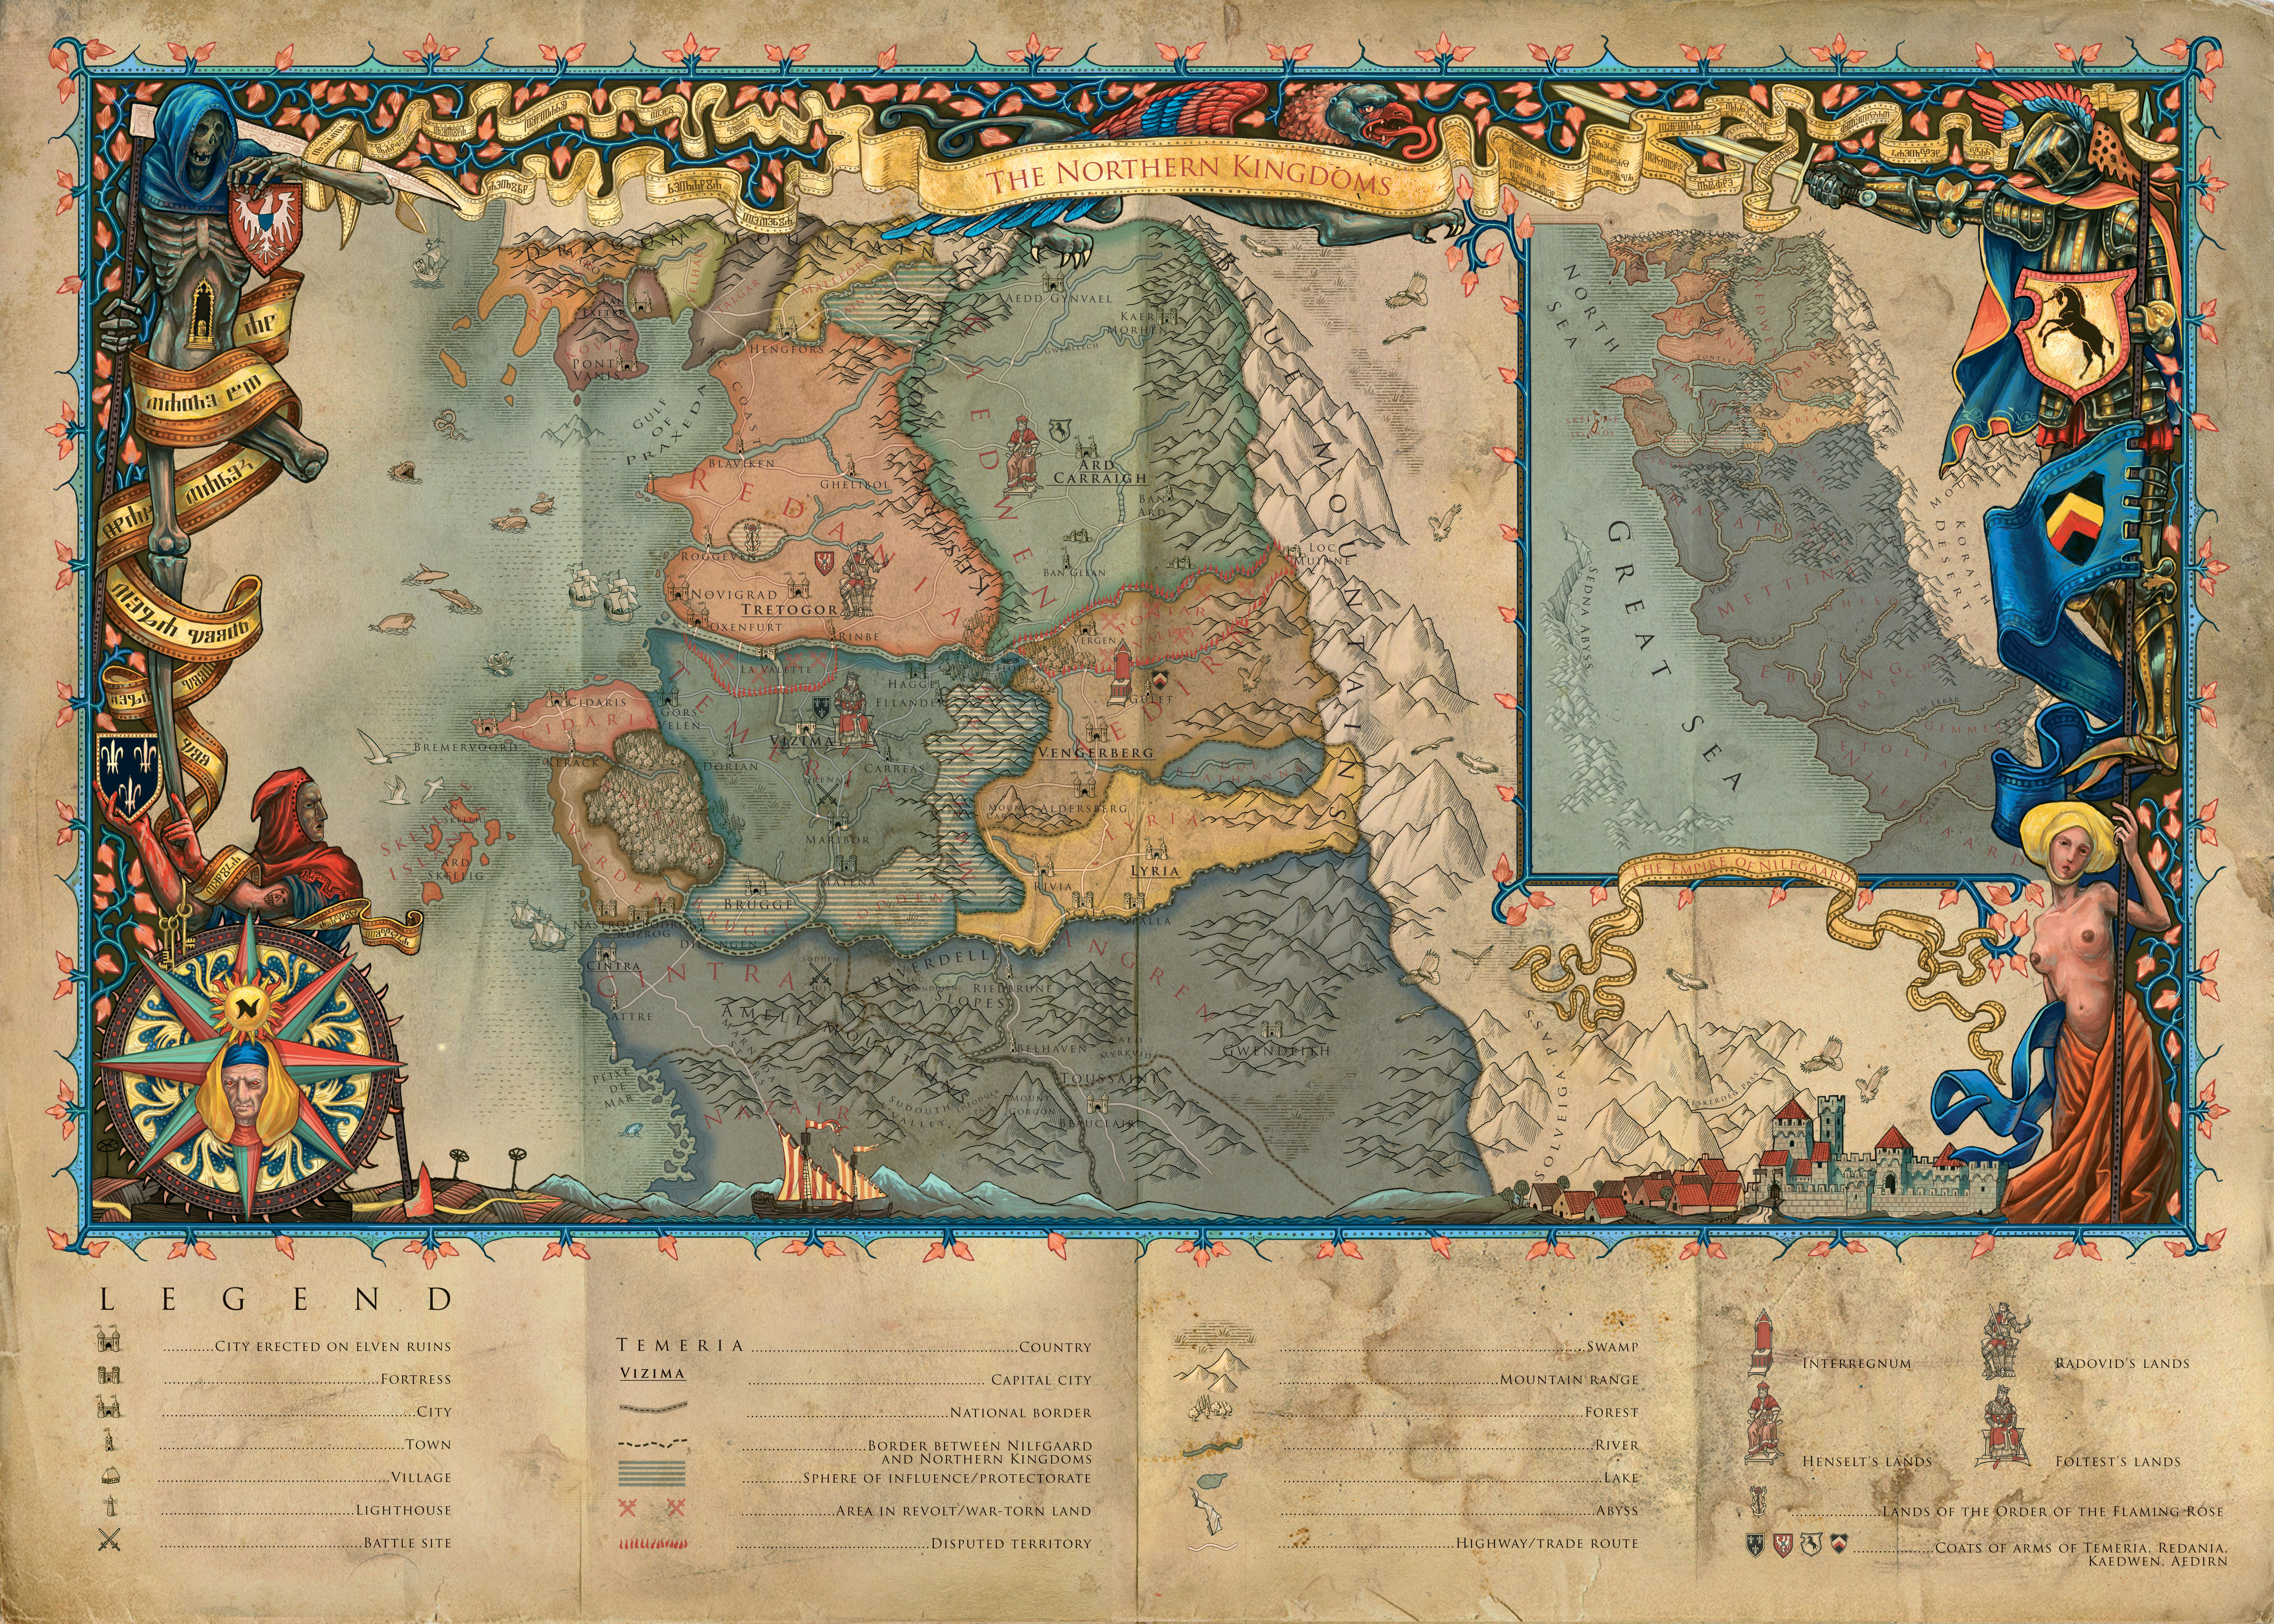
\includegraphics[width=1\textwidth,center]{Northernkingdoms}
	\begin{tiny}\url{https://vignette.wikia.nocookie.net/witcher/images/1/17/Northernkingdoms_full.jpg/revision/latest?cb=20110530105156}\end{tiny}
	\subsection{Wichtige Regionen}
	In diesem Abschnitt wird die politische Situation der nördlichen Köngreiche außer Acht gelassen, er befasst sich lediglich mit geographischen Merkmalen.
	\subsubsection{Die Drachenberge}
	Die nördliche Grenze der Zivilisation. Niemand hat sie je überquert, zumindest nicht zweimal, um zu berichten, was sich auf der anderen Seite befindet. Die Gründe hierfür sind ihre extreme Abgeschiedenheit und die namensgebende Drachenpopulation.

	\subsubsection{Die Blauen Berge}
	Heimat der freien Elfen und natürliche Grenze zu Haakland und Zerrikania. Hier findet sich Dol Blathanna, das Tal der Blumen, eines der Wunder der nördlichen Welt. Die uralte Stadt Loc Muinne, erbaut von den mysteriösen Vran, findet sich auf etwa halber Höhe.

	\subsubsection{Der Pontar und das Pontartal}
	Der Pontar ist einer der größten Flüsse im Norden und trennt das Land von den Blauen Bergen bis zum Meer in einer nahezu horizontalen Linie. Das Tal, dass der Strom sich über die Jahrtausende geschliffen hat, ist das Füllhorn des Nordens: nahezu alle handelbaren Lebensmittel werden hier angebaut, einschließlich den Weinen des Nordens.

	\subsubsection{Die Berge von Mahakam}
	Die Erzreichen Bergkette zieht sich entlang der Grenze von Temeria und Aedirn. Sie ist die Heimat der Zwerge und Gnome und berühmt für deren hochwertige Schmiedekunst. Die größte Siedlung der Berge liegt unter dem Kohlenberg, wo seine Bewohner das weltbeste Eisen abbauen und die Gnome in ihren Werkstätten erstklassige Waffen wie die Gwyhir schmieden.

	\subsubsection{Die Skellige-Inseln}
	Eine Ansammlung von sechs Inseln westlich des Kontinents. Die rauhen Klippen und das graue Meer haben eine ungezähmte Schönheit. Jeder Reisende wünscht sich, einmal in seinem Leben die Sonne von einem Skelliger Gipfel ins Meer sinken zu sehen.

	\subsubsection{Brokilon}
	Von Menschen ``Wald des Todes'' genannt, erstreckt sich die wird die Heimat der Dryaden über das größte Waldgebiet des Nordens. Er bietet all jenen, die von Menschen verfolgt und diskriminiert werden, Zuflucht. Der Wald ist das letzte Reich des Nordens, das nie von Menschen erobert wurde.

	\subsection{Königreiche und Völker}
	\subsubsection{Redania}
	Zur Zeit unter der Herrschaft König Radovid des Strengen, profitiert das Land vom Handel mit den anderen Reichen des Nordens. Die wichtigste Quelle von Redanias Wohlstand sind die Getreideexporte in den restlichen Norden. Die Wirtschaft wird allerdings von billigeren Importen aus Nilfgaard gefährdet. Redania steht in einer langen Tradition des Krieges mit Temeria, allerdings haben die beiden Reiche sich unter Radovids Herrschaft einander angenähert.
	\paragraph{Wichtige Städte}
	\subparagraph{Novigrad}
	Obwohl Novigrad geographisch in Redania liegt, unterliegt sie nicht Radovids Herrschaft sondern ist vollständig selbstverwaltet. Die Stadt ist durch Handel zur reichsten Stadt des Nordens geworden, was sie hauptsächlich ihrem Hafen, einem der größten des Kontinents, zu verdanken hat.\\
	Die Kirche des ewigen Feuers ist in der Freien Stadt so stark wie sonst kaum vertreten, der größte Tempel der Kirche thront auf einer steilen Klippe über der Stadt. Hexenjagden und Feindseligkeit gegenüber Nichtmenschen durchziehen daher die Stadt wie sonst nirgends.\\
	Offiziell wird die Stadt von einem Stadtrat verwaltet, tatsächlich aber liegt sie in der Hand vier krimineller Organisationen:
	\begin{itemize}
		\item Hurensohn Juniors Gruppe, involviert in Glücksspiel, Bordelle und dergleichen
		\item Sigi Reuvens Gruppe, geführt vom ehemaligen Redanischen Agent Sigismund Dijkstra, hält sich im Schatten. Womit genau sie ihr Geld verdienen, ist unbekannt, allerdings liegt die Vermutung nahe, dass es mit Spionage im Großen und im Kleinen zu tun hat.
		\item Die Einwohner der geheimen Straße ``fauliger Hain'' unter der Führung von Francis Bedlam, dem ``König der Bettler''. Die meisten Mitglieder Diebe und Bettler.
		\item Hackers Gruppe, geführt von einem Zwerg, besteht größtenteils aus Zwergen. Sie stellt beinahe eine kleine Armee auf die Beine.
	\end{itemize}
	\subparagraph{Oxenfurt}
	Eine verhältnismäßig kleine Stadt, deren Kern auf einer Insel im Pontar liegt. Berühmt für seine Akademie, die die Naturwissenschaften fördert und den Großteil des Stadtkerns direkt (Campus) oder indirekt (Studentenkneipen\footnote{Wenn jemand ein Problem mit dem grammatikalischen Geschlecht hat, soll er/sie es sich anders denken, an der Oxenfurter Universität studieren auch Frauen, allerdings in der deutlichen Minderheit}) einnimmt. Die Stadt wurde nahezu vollständig auf den Ruinen einer Elfensiedlung erbaut, durch die heute nur noch die Kloake führt.
	\subparagraph{Tretogor}
	Die Hauptstadt Redanias, hauptsächlich für ihr jährliches Pferderennen, das ``Große Tretorianische,'' bekannt.

	\subsubsection{Kaedwen}
	Das größte Königreich des Nordens teilt sich seine Grenzen mit Redania und Aedirn und wird von König Henselt beherrscht. In den letzten Jahrzehnten gab es immer wieder Kriege zwischen Kaedwen und Aedirn, ausgelöst durch den von beiden Seiten erhobenen Anspruch auf das Pontartal. Bis jetzt hält Aedirn diesen Landstrich.
	\paragraph{Wichtige Städte}
	\subparagraph{Ban Ard}
	Die wahrscheinlich wichtigste Stadt Kaedwens. Hier befindet sich die berühmte Magierakademie.
\fi

\chapter{The world}

\subsection{A map of the North}
\begin{center}
	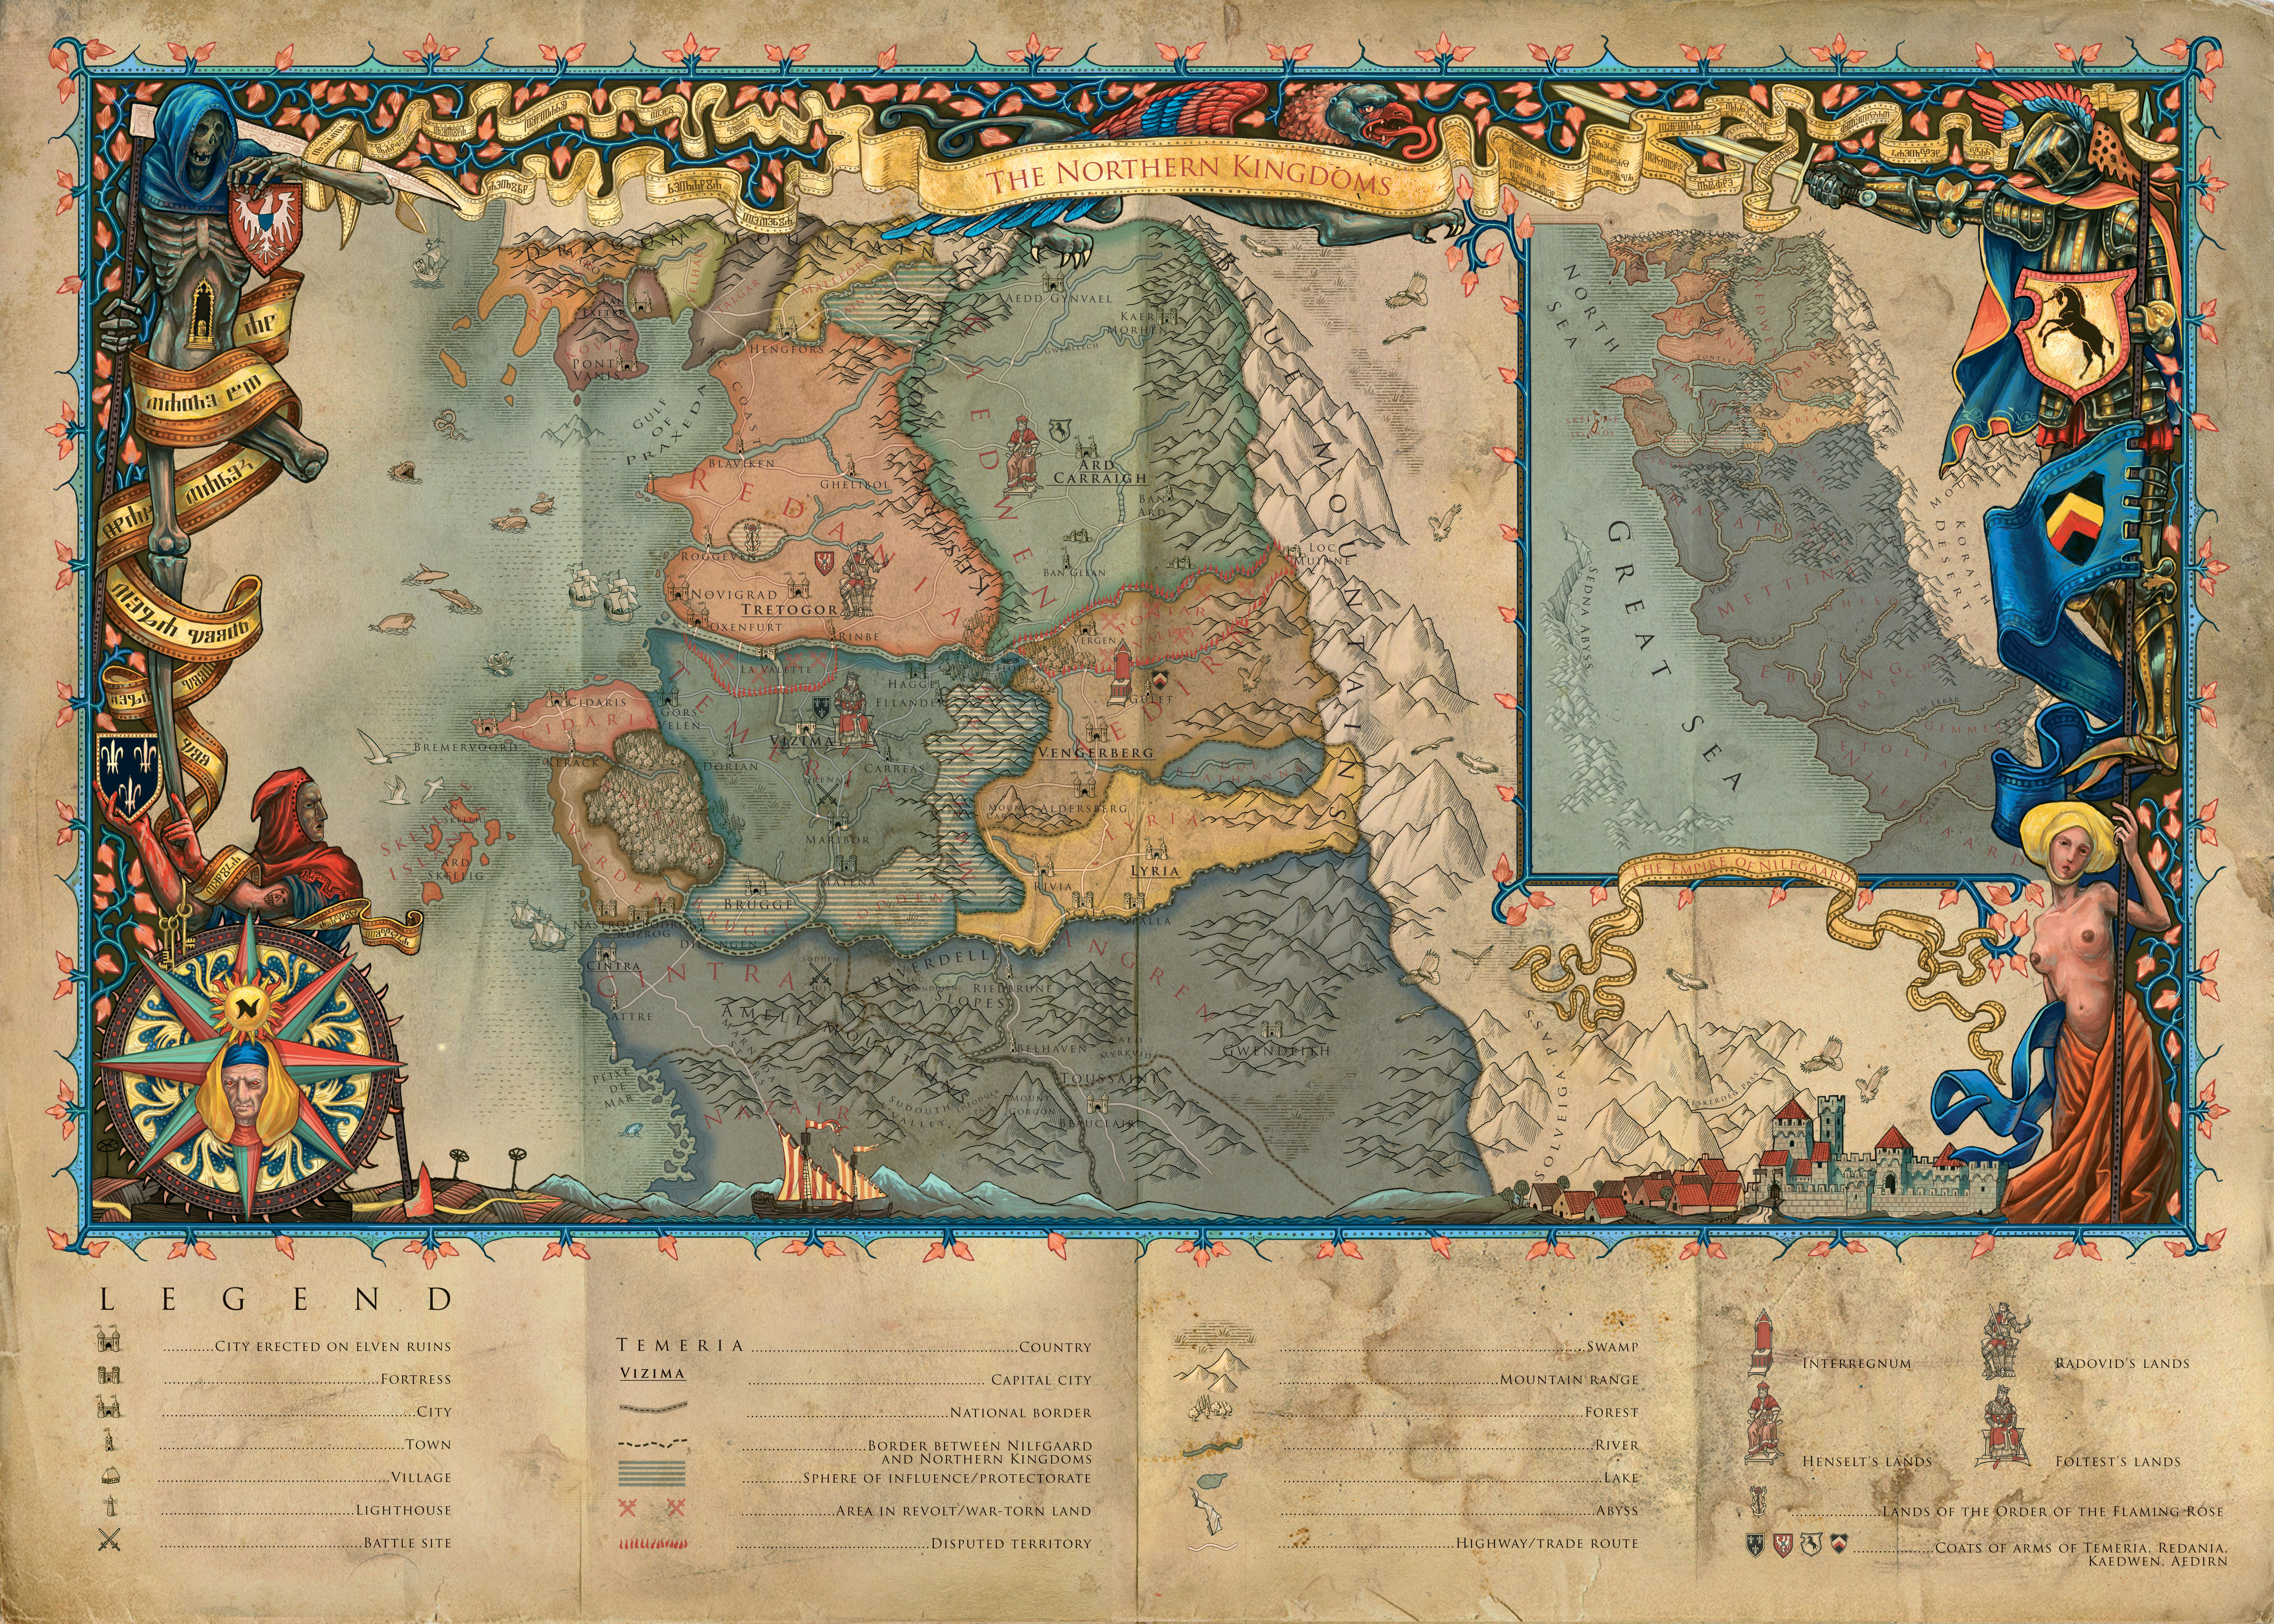
\includegraphics[max size={\textwidth}{\textheight}]{Northernkingdoms}
	\begin{tiny}\url{https://vignette.wikia.nocookie.net/witcher/images/1/17/Northernkingdoms_full.jpg/revision/latest?cb=20110530105156}\end{tiny}
\end{center}

\section{Important regions}\label{region:dragonMtns}
This section ignores the political Situation of the Northern Realms, it is concerned exclusively with geographic features.
\subsection{The Dragon Mountains}
The northern border of civilization. They were never crossed, or at least not crossed twice, so no report of the lands the other side of the mountains has come into the south.
This is explained by their extreme remoteness and the considerable population of dragons the mountain range draws its name from.

\subsection{The Blue Mountains}\label{region:blueMtns}
Home to the free elves and a natural border to Haakland and Zerrikania. Here is Dol Blathanna, the Valley of Flowers, a wonder of the northern world.
Roughly halfway along the range lies the ancient city of Loc Muine that was built by the mysterious Vran.

\subsection{The Pontar River and the Pontar Valley}\label{region:pontar}
The Pontar is one of the chief rivers of the north, seperating the land in a nearly straight line from the \nameref{region:blueMtns} to the sea.
The valley, formed over millenia out of reckoning by the river, is the granary of the north: Nigh on all tradeable foods are grown here,
including the northern wines.

\subsection{The Mountains of Mahakam}\label{region:mahakamMtns}
These mountains form the border between \nameref{realm:aedirn} and \nameref{realm:temeria} and are known for the great wealth
of ore found there. It is hardly surprising that the mountains, homeland of dwarves and gnomes, have produced some of the finest
pieces of smithcraft to be found at this age in the world. The regions largest settlement is situated beneath Mount Carbon,
where its inhabitants mine incessantly for the worlds best iron and gnomes in their smithies forge excellent weapons, such as
the renowned \hyperref[weapon:gwyhir]{Gwyhir}.

\subsection{The Skellige-Isles}\label{region:skellige}
A collection of six islands to the continent's west. Their rough cliffs and grey sea have an untamed, perilous beauty.
No traveller in the north should forgo the sight of the sun sinking into the sea from a summit of a mountain in Skellige.

\subsection{Brokilon}\label{region:brokilon}
Called by men the ``Forest of Death,'' the home of the Dryads stretches across the north's largest wood. It offers a refuge to
all those pursued and discriminated against by men and stands as the last realm never conquered by the younger race.

\subsection{Velen}\label{region:velen}
A miserable province of \nameref{realm:temeria}, to the north of \nameref{city:gors_velen}. The people of this
province are poor and most of it is covered by extensive swamps and dark woods. Travellers are likely to be met
with distrust, if ever they reach a village and do not fall victim to \hyperref[monster:drowner]{drowners} or
brigands.

\newpage

\section{Nations and states}
This section \textit{is} concerned with politics, as well as social structures and institutions.

\printrealm{aedirn}

\printrealm{cintra}

\printrealm{kaedwen}

\printrealm{nilfgaard}

\printrealm{redania}

\printrealm{temeria}

\printrealm{toussaint}

\section{Peoples and groups}
This section will list and describe some of the associations that, while not nations, are perhaps interesting to know about.

\subsection{The clans of \hyperref[region:skellige]{Skellige}}\label{people:skellige}
The inhabitants of the \nameref{region:skellige} are shaped in large part by the isles they inhabit: They are rough, blunt,
and thick-headed, but fierce not only in enmity, but in friendship also. They trust their own strength and boast of their
daring deeds, whether they be successful battle or a long and difficult voyage. Since they live in an archipelago, their culture
is tied closely to seafaring, and they build the dreaded drakkars, longships, which they use in raids against the continent.
These raids are necessary to their economy, since the islands are small and rocky, with little farmland available, but they are
also a kind of sport: While the people on the continent might condemn theft and robbery, you might say a ship-load of \hyperref[people:skellige]{Skalds}
falling upon a small town is a fair contest, and the winner gets to choose their price.
\\[1ex]
Despite centuries of armed conflict, the islanders and the mainlanders don't exactly hate each other, and there is trade with
such goods and services as the one can provide the others - \hyperref[region:skellige]{Skelliger} mercenaries are highly valued,
for example, not only for their skill at arms, but also their honesty and loyalty\footnote{Wich is prone to running out once the coin does}.
\\[1ex]
The women of \hyperref[region:skellige]{Skellige} are trained in warfare alongside the men, likely owing to the men's frequent and prolonged
absences from their homes, and are by law equal in all aspects of life. Nonetheless, it is rare for women to hold a position of authority
in one of the clans.
\\[2ex]
The clans themselves are subdivided into bonds and ruled by one chieftain, the Jarl. In war, all clans are led by one central figure,
elected for life by the jarls: The King of Skellige. His role is purely a military one, though of course a good deal of honour and prestige
come with it, and most of the actual commanding is done by the Jarl of Skellige, the admiral of the islanders' fleet. There are seven clans
inhabiting the chief isles of the archipelago:

\subsubsection{Clan Brokvar}
The descendants of Sove inhabit the north-east of the isle of Spikeroog. Ever since one of their Jarls refused to give battle when outnumbered, they have
been considered cowards by the clans Tuirseach and an Craite, though all admit the archers of Clan Brokvar have no equal on the isles.

\subsubsection{Clan an Craite}
Clan an Craite's seat of power is the citadel of Kaer Trolde, said to have been carved from the rock single-handedly by the clan's founder Grymmdjarr,
from where it's jarls rule the northern half of Ard Skellig. They are the closest ally of Clan Tuirseach.

\subsubsection{Clan Dimun}
Though Clan Dimun claims descent from Broddr, a virtuous hero, their reputation even on the \hyperref[region:skellige]{isles} is one of cheats, thieves
and marauders, and their raids are considered brutal even by \hyperref[region:skellige]{Skellige}-standards. Their Jarls rule the isle of Faroe from Harviken.

\subsubsection{Clan Drummond}
The Clan's original territory was Undvik, but they are now settled in the southern half of Ard Skellig. They claim that Clan an Craite seized the northern half
from them and therefore consider them rivals rather than neighbours. Despite this dispute, it is Clan Heymaey who suffers the most under Clan Drummond, whose
jarls have made a habit of pillaging Hindarsfjall. The Jarls rule from Holmstein and Kaer Muire and consider Modolf their founding father.

\subsection{Clan Heymaey}
The isle of Hindarsfjall is ruled by Clan Heymaey, whose progenitor is seid to be Otkell. The clan stands out from the others by it's piety: The temple of Freya
and the holy grave of Hindar are both located on their island. Aside from traditional skirmishes with raiders of Clan Drummond, Clan Heymaey gets along
very well with the other clans.

\subsection{Clan Tordarroch}
The ancestral home of Clan Tordarroch is on Undvik, but they have recently removed from the island to live in their ships: an ice giant has driven them from
the isle and made it uninhabitable, they claim. Over time, their ships were bridged with more and more planks, until eventually, they were all a single structure:
The Floating Market.

\subsection{Clan Tuirseach}
The descendants of Tyr rule An Skellig, the island best-suited for farming, since it has a wide and enclosed plain where crops are relatively sheltered from the
sea. This clan has brought fourth more kings than any of the others, and they are greatly strengthened by their alliance with Clan an Craite.

\subsection{The Order of the Flaming Rose}

\subsection{The Witch-hunters}

\section{Religious cults}

\subsection{The cult of Freya}\label{religion:freya}

\subsection{The church of the Eternal Fire}\label{religion:eternal_fire}

\section{Customs}

\subsection{The Law of Surprise}
In the north, it is the custom that if one man by chance comes upon another in distress and saves his life, they should not go unrewarded, but neither
should the saviour be greedy in choosing his boon. Instead, the Law of Surprise is invoked: ``Give me that which you find at home but did not expect.''
This may be as little as a dead dog who was still alive when the owner left, but in some tragic cases, men have returned home to find their wives pregnant.
The Law is held sacred, and people are loth to break it.

\chapter{Character creation}
In this chapter, the impact of the characters race on stats and gameplay will be described. A short and intentionally vague paragraph on starting
equipment is also included after each ``class''. These are only suggestions and not meant to be exhaustive, anyone playing this plugin is likely
to know the franchise well enough to figure out for themselves what is reasonable equipment.

\section{Race}
A character's race has little influence over their stats, instead, the chief effect it has is a social one: Humans, particularly in the North,
pursue and dislike any of the other races, though the extremity varies from area to area. An elf may be well-advised to cover his ears when
taking a stroll around \hyperref[city:novigrad]{Novigrad}, whereas a human will be in deep trouble when trespassing into \nameref{region:brokilon}.
Discrimination needn't be limited to open hostility, however: A cunning narrator will perhaps charge a dwarf double when he tries to shop in
human territory.

\subsection{Elves}
Elves appear somewhat feminine regardless of gender, their ears are pointed and they seldom
wear beards. They have a knack for plants and animals, and are rarely seen in metal armor.
\\\\
Elves gain one additional attribute point in REF, as well as a bonus success to perception.

\subsection{Dopplers}
Dopplers live a dangerous life: Should they be found out, most would burn them at the stake or try to exploit them in criminal endeavours.
They can take the shape of any humanoid creature\footnote{Whose size is not too different to their own, roughly from 80cm to 280cm} they have seen before, which not only makes them look practically identical but also allows the
doppler to use some of their skills. Any permanent markings on the body, such as scars or tattoos, will be present in any form the doppler takes.
The doppler may not change his shape while touching silver, and cannot create silver accessories. Clothes and the like can be manifested,
but turn into unsightly lumps of flesh when out of contact with the doppler's body.
\\\\
Dopplers don't gain any points by default, but may \textit{transform}. When transformed into another character, their effective skill points in
any skill\footnote{Explicitly not in attributes} are the average between their own and those of whoever they impersonate. They are, unless marked
by some permanent feature, indistinguishable from the people they copy, but may still be found out if they behave strangely.

\subsection{Dwarves}
Dwarves are shorter than humans, but typically a bit taller than halflings. They make excellent
heavy infantry, but can also be prolific craftsmen. It should also be mentioned that the world's
largest bank is run by the Vivaldis, a family of dwarves.
\\\\
Dwarves gain one additional attribute point in STR, one extra success in grappling and no penalty
when unarmed in close combat.

\subsection{Halflings}
Halflings, as a rule, are on better terms with humans than most other races. One possible explanation for this is that they tend to live
in secluded farmsteads and keep out of the way of humans while supplying them with honey, roots and other agricultural commodities.
\\\\
Halflings may roll one extra die on \textit{aim/throw}, \textit{acrobatics} and \textit{sleight of hand} checks, and they are immune to magic%
\footnote{This includes hypnosis and the like. Magic can still harm them, as, for example, while they cannot be magically set ablaze, their surroundings
	can, and they are not immune to heat. Nor large rocks, for that matter.}. They must not exceed one attribute point in STR.

\subsection{Humans}
Since Cogent Roleplay assumes humans as the standard, so shall this plugin. Humans' stats are simply the default,
but they will not draw any special attention to themselves in most regions. If some advice may be given, it makes
for a less interesting game to pick one's character by giving them the best stats possible than by coming up with
a character concept and picking skills consistent with that concept.

\section{Professions}
Naturally, the typical professions found in most fantasy settings can be applied here, too; it is advised, however, to talk over specifics with
the narrator, as social positions might be and organizations will be unique to this world. Since this document should allow even those with no
prior experience of The Witcher at least to participate in a campaign, some of the less obvious professions are listed here.

\subsection{Havekar}
Smugglers who sell arms to the \nameref{profession:scoiatael}, some out of sympathy but most out of greed. They are scarcely less hated than the ones they supply,
and slightingly named Hawkers by their enemies. Their equipment need not differ greatly\footnote{Or even at all} from that of other men of similar
wealth, which, in turn, could reasonably range from 3 to 5.

\subsection{Scoia'tael}\label{profession:scoiatael}
Guerrilla fighters in league with \nameref{realm:nilfgaard}, they joined the second northern war to fight for a free country of non-humans.
They are mostly elves and dwarves, but some halflings have also joined the ranks. Even now, in times of peace, they continue to harass the
unwary, turning more and more into terrorists. Men call them Squirrels and pay good money for their heads. High-ranking Scoia'tael are
likely to wield a \hyperref[weapon:gwyhir]{Gwyhir}, but light armour, sword and bow are likely part of any Guerilla's equipment.
They should not start out with wealth above the equivalent of two commerce points.

\subsection{Knight-errant}\label{profession:knight_errant}
Well-armed, usually noble-born cavalrymen in the service of the dukes of \nameref{realm:toussaint}. They value their honour over their lives and are
bound only by their word. In \nameref{realm:toussaint}, they serve as a free police-force, envoys to other states and keepers of the peace in general.
Younger Knights-errant in particular are drawn to acts of foolish grandeur, such as taking on monsters on their own and without any silver. Within
\nameref{realm:toussaint}, they are easy enough to find, but they will need a very good reason to venture beyond the \hyperref[realm:toussaint]{duchy's} border.
A Knight-errant should start out with full body armour, a (possibly armoured) horse, a sword as backup and a primary battle weapon such as a lance or
a bow. Their starting wealth should not exceed the equivalent of five or six commerce points, nor go below the equivalent of three.

\section{Witchers}
Since being a Witcher determines both one's profession and genetic makeup, they will be treated separately from all other types of character. Quite appropriately,
when you think about it.
\\\\
Witchers, similarly to non-humans, suffer distrust and harassment in most places, especially cities far removed from the monsters Witchers were
made to combat. They are generally tolerated, however, much in the way that whalers are: They're nasty, unrefined, and they stink, but their
jobs have to be done by someone. It is also commonly accepted that the mutations Witchers undergo rob them of any emotions. Their eyes are like
those of a cat, and by this, they can be told from regular humans, if the two swords did not already give the game away.
\\\\
Witchers gain one additional attribute point to be spent on either STR or REF. Their vocation is \textit{Witcher}%
\footnote{This vocation can be used to assist in most perception checks, as it includes the Witchers' senses.
	It also includes herblore, knowledge about monsters and all things part of the profession}
, and they must put at least two skill points into this vocation, as well as one skill point each into proficiency with longsword
and \hyperref[rule:signs]{signs}. Witchers needn't make any dice rolls to determine their compatibility with \nameref{rule:witcher_potions}.
\\\\
Starting wealth will typically range from 1 to 3. The Witcher will likely be equipped with light or medium armor, a steel and a silver
longsword and perhaps one or two potions.

\subsection{Witcher schools}
In the hay-day of witcherdom, several schools for training the next generation of witchers were strewn across the land.
These days, however, their fortresses lie are ruined and desolate, the once-great schools reduced to a handful of vagabonds
and the secrets of the mutations all but forgotten. Still the roving witchers are associated with their respective schools
by the shape of their medallions, a stylized head of the animal that gave the school it's name.

\paragraph{School of the Bear:}
The first school to split off from the more ancient Order of Witchers established their base in the Amell Mountains by \nameref{realm:cintra}
After failing to rid the area of a cabal of vampires, the local villager's frustration boiled over and the witchers,
feeling no great loyalty to their school or each other, dissolved the school and abandoned the fortress. It is supposed
that some of the former bears still rest there from time to time, though the castle has long lain in ruin.

\paragraph{School of the Cat:}
After an internal conflict which destroyed their castle in the south, the rag-tag leftovers formed into the Dyn Marv Caravan and embraced nomadship.
They hired themselves out to anyone for any job, so long as the pay was good. Like the Wolves, they were betrayed and nearly
destroyed by king Radowit II. in an attempt to secure his power.

\paragraph{School of the Griffin:}
The School of the Griffin most closely retains the code of the ancient Order of Witchers that predated all the schools:
Alongside swordcraft and alchemy, young Griffins are educated in etiquette. Their castle was Kaer Seren in Kovir, but it was
badly damaged in a feud with envious mages who summoned a landslide in the mountains above it. Griffins, unlike all other
witchers, are not averse to slaying dragons.

\paragraph{School of the Viper:}
The Vipers split from the School of the Bear soon after its foundation and moved south, into \nameref{realm:nilfgaard}.
They accepted contracts on humans as well as monsters, though their purpose was another: to defeat the Wild Hunt.
When they refused to enter the service of the Usurper, he ordered his armies to destroy their keep, scattering the students.
They have since been banned from entering any city large enough to enforce this edict.

\paragraph{School of the Wolf:}
Once occupying the fortress of Kaer Morhen in the \nameref{region:blueMtns}, the Wolves fell victim to a pogrom roused by
mages and priests that destroyed their home and their order. Now the keep only serves as a place for the last remnants of
the school to spend the winter.

\chapter{Magic system}
\section{Witcher signs}\label{rule:signs}
A Witcher may cast these signs as long as he has at least one free hand. If he casts one of these signs in
combat, their base modifier is +0D6.

\subsection{Aard}
The character issues a shockwave from their hand. Can replace strength checks (use two thirds of successes).

\subparagraph{In combat:} Cannot damage opponents, but only \textit{stagger}, \textit{disarm} or \textit{trip}. Add 2 successes.

\subsection{Axii}
Mild form of hypnosis. May be used to assist in persuasion, deception or any other skill attempting to influence
someone's mind. Some monsters and most mages are immune to such manipulation.

\subparagraph{In combat:} Detract victory level over victim from victim's successes next turn. If the victim's
successes thereby become negative, they are doubled to assault their partners (if any).

\subsection{Igni}
The character issues small amounts of flame from their hand. Can be used to light fires, candles etc.

\subparagraph{In combat:} +1D6 in close combat. The player may choose to blind the opponent
if he achieves a victory level of 3 or higher.

\subsection{Quen}
The character draws up a shield around themselves. This protects them from fire as well as small objects, such threats as
falling trees, for example, are not averted by Quen. The shield fits one character for every 2 successes rolled.

\subparagraph{In combat:} Purely defensive round, but the successes are doubled.

\subsection{Yrden}
The character sets up a magical trap in a circle 1 or 7 feet in diameter. They must be able to pysically reach the perimeter to do this. Only one such trap may be active at any one time.

\textbf{Small circle:} The first opponent to step into the circle is immobilized for one turn of combat for every success above 3.

\textbf{Large circle (CL4):} Every opponent within the circle rolls one fewer die on every roll.

\nameref{monster:spectre} may be harmed by any weapon while within a trap set by Yrden.

\subparagraph{In combat:} Setting up a small circle takes one turn of combat, the large circle takes three.

\section{Witcher potions}\label{rule:witcher_potions}
The potions' effects typically last about 8 hours.

If any non-Witcher tries taking a Witcher potion, they must make a destiny roll. If this roll is an eight or worse,
they are poisoned by the potion, the severity ranging from day-long nausea to incapacitation and serious risk of death,
unless medical action is taken. If the result ranges from nine to twelve, the character drinking the potion throws it
up but suffers no long-term damage from it. If the result is thirteen or higher, the potion developes its effect
partially or fully.

A Witcher attempting to consume more than 3 potions in 36 hours is treated like any non-Witcher for every potion he drinks
after his third.

Penalties for repeated incompatability may be issued as seems fit.
\\[2ex]
\subparagraph{Rarity of ingredients:}
The rarity of ingredients determines the challenge level on a survival check on finding them in the wild%
\footnote{Though, of course, depending on one's surroundings, penalties or boni may be issued}.
It should also inform the availability and cost when attempting to purchase them.

\subsection{Black blood}
Turns the consumer's blood into a lethal poison. Any creature drinking it while the effect lasts immediately receives
poisoning equivalent to a level 4 injury.
\\[2ex]
Rarity of ingredients: 3

\subsection{Cat}
Negates all penalties to perception checks caused by darkness.
\\[2ex]
Rarity of ingredients: 2

\subsection{Killer Whale}
Significantly raises the body's ability to absorb oxygen. Doubles the time the consumer can spend without breathing,
if they drank the potion at least ten minutes beforehand.
\\[2ex]
Rarity of ingredients: 2

\subsection{Swallow}
Immediately heals all level 1 injuries. Over time reduces the injury levels of all injuries by up to 2.
\\[2ex]
Rarity of ingredients: 4

\subsection{Thunderbolt}
Grants one extra die for each combat roll, but negates boni for defensive actions.
\\[2ex]
Rarity of ingredients: 4

\subsection{White honey}
Cancels the effects of all other potions and removes any poisoning caused by them.
\\[2ex]
Rarity of ingredients: 3

\section{Runes}
Weapons and armor may be inlaid with runes by some skilfull craftsmen, at a price equivalent to
3 commerce points. These runes provide minor boni, but are mutually exclusive\footnote{One balanced way
	to get around this restriction might be to have an exceptionally skilled craftsman who can inscribe
	sets of runes, but takes much higher prices.}.
The system assumes the use of the harcore combat rules, though it may be adapted to a regular game.

\begin{itemize}
	\item \textbf{Rún de gearradh:} +1D6 to any weapon that already provides at least 2D6 weapon bonus.
	\item \textbf{Rún de tolladh:} A weapon that already reduces the opponent's armor level reduces it
	      by one additional level if inlaid with these runes.
	\item \textbf{Rún de éaradh:} These runes create a forceful push when the weapon they're inscribed
	      on impacts a target. +1D6 aditionally when declaring to stagger, disarm or trip.
\end{itemize}

\chapter{Special items}
\section{Weapons}
These are some particular weapons which, technically, fall into one of the categories of the Cogent rule book,
but receive superior stats to reflect their renown within the world.

\weapon[weapon:gwyhir]{Gwyhir}{Forged by cunning gnomes in the deep smithies of Mount Carbon, these swords
	are widely considered the best to be bought for money.}{3}{3}

\chapter{Detailed currencies}
Since haggling can be quite fun, and makes much more sense when playing with actual numbers than with commerce points%
\footnote{Raising the reward for taking care of some monster from the price of a sword to the price of a house, for instance,
	is rather unrealistic},
here is a proposal for a more detailed financial system. To make it more realistic (and true to the games), different nations
will use different coinage, so travel may well include some measure of exchanging one currency to another. For the player's
convenience, the narrator may simply pick the coinage they like best and pretend it were universal.
\\[2ex]
Since there is already some level of complexity within each currency, it may be most convenient to simply split one's
wealth into copper, silver and gold coins as is usual elsewhere and keep in mind the conversions between the metals.
If one currency is to be converted to another, different rates may be applied to different metals, so one should not simply
add a silver coin if one has gained the appropriate number of coppers - an actual exchange is needed. Additionally,
coins have weight. The narrator may apply penalties for carrying to many coins, so higher denominations can be important
if large purchases are to be made.
\\[2ex]
I want to be very clear about the fact that the coins listed below were, aside from the three well-known ones, invented
or at least introduced to the world of the Witcher by me. They are not canon and may, in some cases, even conflict
with the canon, but I have taken the liberty to create systems of coinage which I find at least credible both within
the context of the Witcher and without it. My hope is that asking for two trees will be more immersive than asking
for twenty copper-pieces, and also that the handful of names necessary to play in one location are not too many to
remember.

\section{\hyperref[realm:temeria]{Temerian} coinage}
The most well-known \hyperref[realm:temeria]{Temerian} coin is doubtlessly the crown. Making this the \textit{only}
\hyperref[realm:temeria]{Temerian} coin, however, would be blatantly ignorant of actual systems of currenty as well
as simple practicality. Here, then, is the full system:

\begin{itemize}
	\item \textbf{Studs:} Small copper coins, named in times long past after the studs on the crown of Temeria.
	      Their original name no one now recalls. Four studs will buy a hot meal or a bed in an inn for a night.
	\item \textbf{Trees:} Large copper coins, named after the large tree-shapes on the crown of Temeria. Trees are
	      the value and weight of ten studs.
	\item \textbf{Crowns:} Small silver coins, valued at 60 studs. A crown's worth of studs weighs precisely half
	      a \hyperref[realm:temeria]{Temerian} pound. Expensive swords may cost around one crown, perhaps more if made by renowned craftsmen or decorated lavishly.
	\item \textbf{Towers:} Silver coins the weight and value of 24 crowns, named for the depiction of \nameref{city:vizima}'s
	      chief gate impressed on them, on which a tower features prominently.
	\item \textbf{Royal crowns:} Small gold coins, valued at 120 crowns. Officially, they are called eagles, but since for
	      a long time only nobility dealt in large enough sums to need these, they were commonly called  `Nobleman's crowns',
	      `King's crowns' or `royal crowns'. The latter name stuck.
\end{itemize}

\section{\hyperref[realm:redania]{Redanian} coinage}
What the crown is for \nameref{realm:temeria}, the oren is for \nameref{realm:redania}. For the reasons explained above,
here is a more detailed set of denominations.

\begin{itemize}
	\item \textbf{Pennies:} Small copper coins, of similar value to the Temerian studs\footnote{Conversion rates may differ and change, of course}.
	\item \textbf{Guinnies:} Medium sized copper coins. They are the exact weight and value of 12 pennies.
	\item \textbf{Hierarchs:} Large copper coins, first commissioned by a hierach of \hyperref[city:novigrad]{Novigrad} to
	      be the precise weight and value of 36 pence.
	\item \textbf{Orens:} Medium sized silver coins, valued at 240 pence. An oren's worth of pennies weighs precisely one
	      \hyperref[realm:redania]{Redanian} pound.
	\item \textbf{Barges:} Small gold coin with an impression of a trade ship, commissioned by the \hyperref[city:novigrad]{Novigrad}
	      city council to celebrate their new-found wealth soon after the city gained independence. A barge is valued at 24 orens.
\end{itemize}

\section{\hyperref[realm:nilfgaard]{Nilfgaardian} coinage}
The `\hyperref[realm:nilfgaard]{Nilfgaardian} crown' is the floren. Below is a list of further coins.

\begin{itemize}
	\item \textbf{Silans:} Very small copper coins of about half the weight and purchasing power of the \hyperref[realm:temeria]{Temerian}
	      stud.
	\item \textbf{Deniers:} Small copper coins. They are the exact weight and value of 4 Silans.
	\item \textbf{Petalens:} Large copper coins. They are the exact weight and value of 100 Silans.
	\item \textbf{Florens:} Medium sized silver coins, valued at 500 Silans. A Floren's worth of Silans weighs
	      precisely 500 \hyperref[realm:nilfgaard]{Nilfgaardian} grams.
	\item \textbf{Usurper's gold:} Very small gold coins with an impression of the Usurper's face. Valued at 20 Florens.
	\item \textbf{Suns:} Small gold coins, valued at 50 Florens.
\end{itemize}

\chapter{Additional combat modifiers}

\large

\subsubsection*{Positive}

\rowcolors{2}{tablebackgroundpos2}{tablebackgroundpos1}
\begin{tabularx}{\textwidth}{cX}
	\rowcolor{tablebackgroundposhead}
	\textbf{Name} & \textbf{Effect} \\
\end{tabularx}


\subsubsection*{Negative}

\rowcolors{2}{tablebackgroundneg2}{tablebackgroundneg1}
\begin{tabularx}{\textwidth}{cX}
	\rowcolor{tablebackgroundneghead}
	\textbf{Name}                       & \textbf{Effect}                                                  \\
	Blindness\label{modifier:blindness} & -4D6, Destiny roll to determine target of attack.                \\
	Swimming\label{modifier:swimming}   & -2D6 to throw-checks, -3D6 in combat. Large bows cannot be used. \\
	Submerged\label{modifier:submerged} & Throwing or using ranged weapons is impossible, -3D6 in combat.
	-1D6 additionally for every two turns spent under water.                                               \\
\end{tabularx}

\normalsize

\chapter{Bestiary}
In this chapter will be listed some of the typical monsters one might face in the world of The Witcher.
Stats are, once again, only suggestions

\section{Beasts}
While not magical in the ordinary sense of the word, these wild animals pose a serious threat to any wanderer
foolish enough to disturb them.

\printmonster{bear}
\printmonster{warg}
\printmonster{wolf}

\section{Humanoids}
These are the various monsters of human shape prowling the world.

\printmonster{harpy}

\section{Necrophages}\label{monster:necrophage}
Here are listed the manifold corpse-eaters plagueing the war-torn areas of the North. Whereever there
are corpses unburied, one can be sure to come across a handful of these truly unsanitory creatures.
\\[1.5ex]
The levels of severity of injuries against necrophages dealt by non-silver weapons are halved.

\printmonster{drowned_dead}
\printmonster{drowner}
\printmonster{mucknixer}
\printmonster{rotfiend}

\section{Relicts}
The creatures described here have but one thing in common: their exceeding rarity. Shortly after the Conjunction
of Spheres, they were abundant on the continent, but when the humans arrived, these species retreated ever further,
until their territories could no longer sustain them. It has been hypothesized that the creatures of this type, or
at least some of them, inhabited the continent before the Conjunction, this is, however, unconfirmed.

\printmonster{fiend}

\section{Spectres}\label{monster:spectre}
This section contains all those incorporeal beings whose origins can be found in the deceased. They cannot be
harmed unless by silver weapons or specialized magic. The weaker ones can be dispelled by silver, but those
with uncut ties to the world of the living may simply reappear the next day if defeated.

\printmonster{noonwraith}
\printmonster{nightwraith}

\chapter{List of abilities}

\abilitylist

\end{document}